\section{Videojuegos lúdicos}

Los videojuegos se utilizan como herramienta educativa que permite a los estudiantes desarrollar competencias en sus procesos de aprendizaje. Informes del Horizon (New Media Consortium) como \cite[Games and gamification]{vid07} resaltan la gamificación como una de las principales herramientas de aprendizaje con mayor crecimiento.
\\[1pt]

Instintivamente, el ser humano aprende jugando. Desde los primeros años de vida el niño adquiere conocimientos a través del juego. Para la psicóloga infantil, esta característica permite al infante socializar en un entorno completamente nuevo, que lo estimula a conocer muchos aspectos de la realidad. Además de ser emocionante y entretenido le permite desarrollar un nivel de pensamiento creativo para enfrentar las circunstancias de la vida. El adulto tiene temor a equivocarse, mientras que un niño juega, se equivoca, lo vuelve a intentar, y de esa experiencia aprende.
\\[1pt]

El videojuego se puede utilizar como un instrumento del proceso enseñanza-aprendizaje. Según lo anterior por el Dr. Francisco Revuelta, especialista en procesos de formación en espacios virtuales dentro del ámbito pedagógico, este es dividido en dos vertientes. La primera, como un simulador de aprendizaje o herramienta en el cual se puede comprobar el nivel de competencia del alumno de acuerdo a las exigencias que le propone el videojuego. La segunda, como un entorno virtual de aprendizaje donde el estudiante es motivado a resolver problemas académicos interactuando dentro del espacio brindado por el videojuego\cite{vid06}. Lo anterior se puede encontrar como ejemplo los siguientes juegos de la imagen \ref{fig:vidLud}.
\\[1pt]
\begin{figure}
	\centering
	\subfloat[Simulador de aprendizaje: Minecraft education edition]{
		\label{fig:mine}
		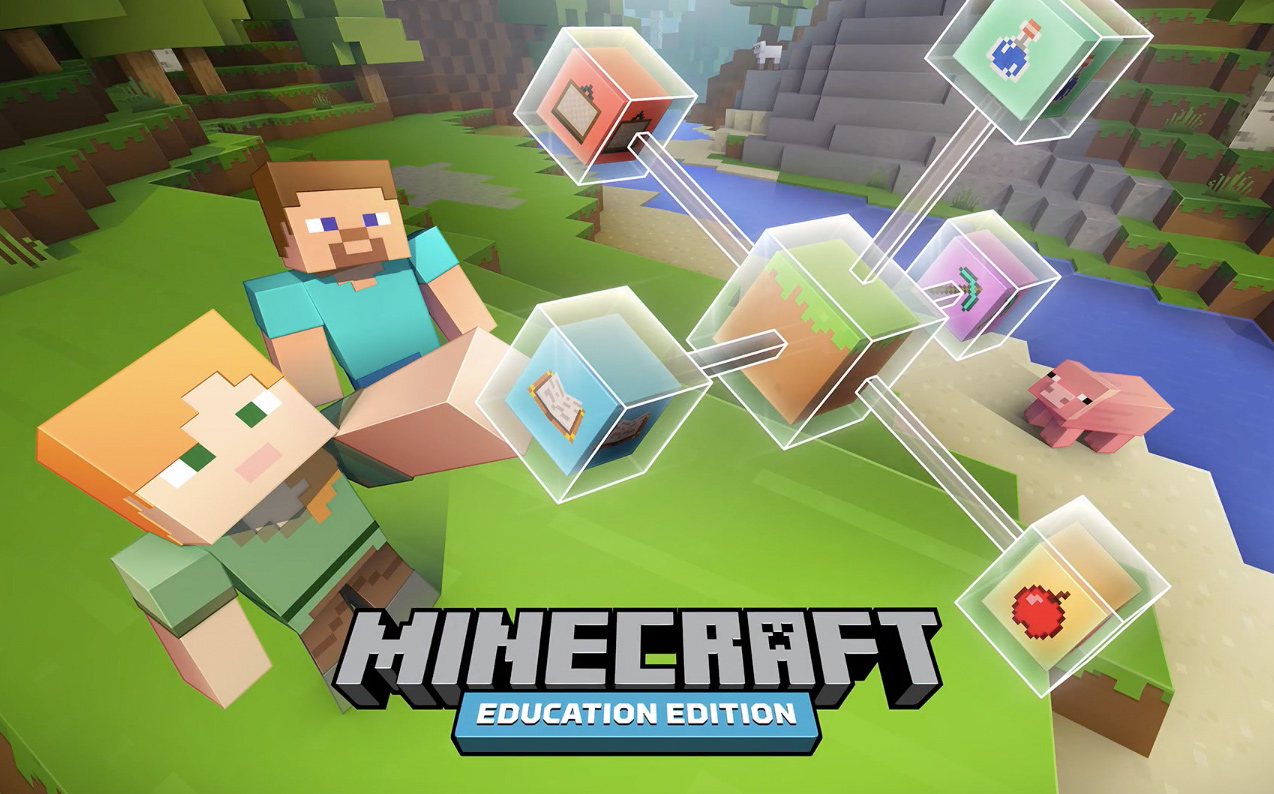
\includegraphics[width=0.5\textwidth]{03MarcoTeorico/imageR/minecraft.jpg}}
	\subfloat[Entorno virtual: Plataforma learny]{
		\label{fig:lea}
		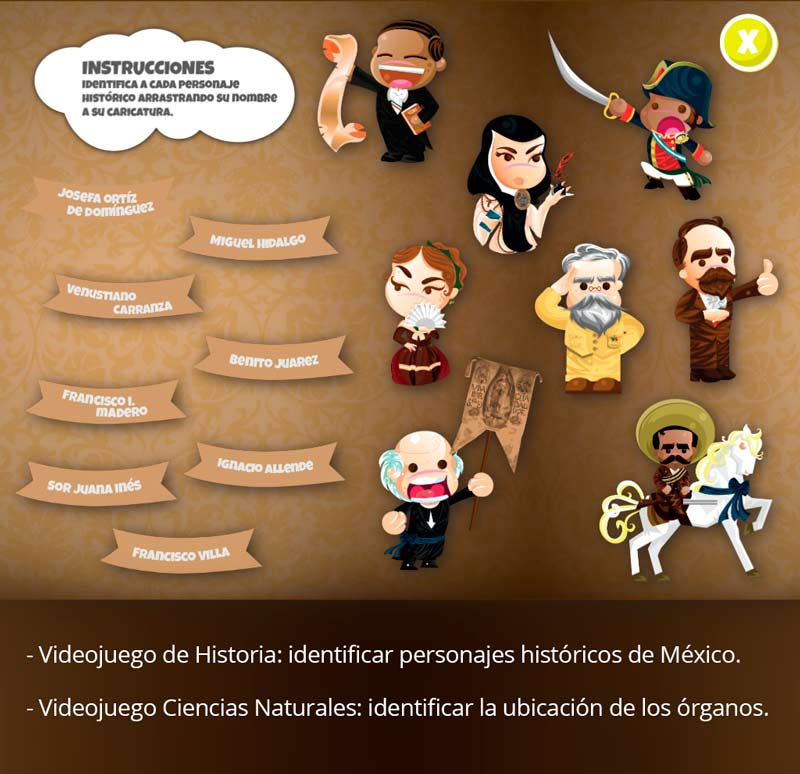
\includegraphics[width=0.5\textwidth]{03MarcoTeorico/imageR/learny.jpg}}
	\caption{Ejemplos de las dos vertientes de videojuegos lúdicos}
	\label{fig:vidLud}
\end{figure}

Dentro de la gamificación el videojuego aumenta la motivación en el aprendizaje, ayuda al alumno a adquirir conocimientos de una manera atractiva y contribuye al desarrollo de competencias. Para que el alumno aprenda, el docente debe plantearse, como primer paso, qué es lo que quiere enseñar y, de acuerdo a esto, se busca un videojuego que sirva de instrumento para motivar el aprendizaje. El videojuego aumenta la motivación en el aprendizaje, ayuda al alumno a adquirir conocimientos de una manera atractiva y contribuye al desarrollo de competencias, pero sólo sirve como complemento de las herramientas básicas en el proceso de enseñanza-aprendizaje.
\\[1pt]
